%
\documentclass[12pt]{article}

% The usual packages
\usepackage{fullpage}
\usepackage{breakcites}
\usepackage{setspace}
\usepackage{endnotes}
\usepackage{float}
\usepackage{amsmath}
\usepackage{amsfonts}
\usepackage{amssymb}
\usepackage{rotating}
\usepackage{dcolumn}
\usepackage{longtable}
\usepackage{microtype}
\usepackage{graphicx}
\usepackage{hyperref}
%\usepackage[usenames,dvipsnames]{color}
\usepackage{url}
\usepackage{natbib}
\usepackage{framed}
\usepackage{epigraph}
\usepackage{lipsum}
\usepackage[font=small,labelfont=sc]{caption}
\restylefloat{table}
\bibpunct{(}{)}{;}{a}{}{,}

% Set paragraph spacing the way I like
\parskip=0pt
\parindent=20pt

% Define mathematical results
\newtheorem{lemma}{Lemma}
\newtheorem{proposition}{Proposition}
\newtheorem{theorem}{Theorem}
\newtheorem{claim}{Claim}
\newenvironment{proof}[1][Proof]{\begin{trivlist}
\item[\hskip \labelsep {\bfseries #1}]}{\end{trivlist}}
\newenvironment{definition}[1][Definition]{\begin{trivlist}
\item[\hskip \labelsep {\bfseries #1}]}{\end{trivlist}}
\newenvironment{example}[1][Example]{\begin{trivlist}
\item[\hskip \labelsep {\bfseries #1}]}{\end{trivlist}}
\newenvironment{remark}[1][Remark]{\begin{trivlist}
\item[\hskip \labelsep {\bfseries #1}]}{\end{trivlist}}

%% Set up fonts the way I like
%\usepackage{tgpagella}
%\usepackage[T1]{fontenc}
%\usepackage[bitstream-charter]{mathdesign}

%\usepackage{helvet}
\usepackage[labelfont={bf}, margin=0cm, font=small, skip=0pt]{caption}

% Baskervald
%\usepackage[lf]{Baskervaldx} % lining figures
%\usepackage[bigdelims,vvarbb]{newtxmath} % math italic letters from Nimbus Roman
%\usepackage[cal=boondoxo]{mathalfa} % mathcal from STIX, unslanted a bit
%\renewcommand*\oldstylenums[1]{\textosf{#1}}

\usepackage[T1]{fontenc}
\usepackage{newtxtext,newtxmath}


%% Set up lists the way I like
% Redefine the first level
\renewcommand{\theenumi}{\arabic{enumi}.}
\renewcommand{\labelenumi}{\theenumi}
% Redefine the second level
\renewcommand{\theenumii}{\alph{enumii}.}
\renewcommand{\labelenumii}{\theenumii}
% Redefine the third level
\renewcommand{\theenumiii}{\roman{enumiii}.}
\renewcommand{\labelenumiii}{\theenumiii}
% Redefine the fourth level
\renewcommand{\theenumiv}{\Alph{enumiv}.}
\renewcommand{\labelenumiv}{\theenumiv}
% Eliminate spacing around lists
\usepackage{enumitem}
\setlist{nolistsep}

% Create footnote command so that my name
% has an asterisk rather than a one.
\long\def\symbolfootnote[#1]#2{\begingroup%
\def\thefootnote{\fnsymbol{footnote}}\footnote[#1]{#2}\endgroup}

% Create the colors I want
\usepackage{color}
\definecolor{darkred}{RGB}{100,0,0}

\hypersetup{
 pdftitle={Logistic Regression in Small Samples}, % title
 pdfauthor={Kelly McCaskey and Carlisle Rainey}, % author
 pdfkeywords={logit}{probit}{logistic regression} {small sample} {bias}{bootstrap},
 pdfnewwindow=true, % links in new window
 colorlinks=true, % false: boxed links; true: colored links
 linkcolor=black, % color of internal links
 citecolor=black, % color of links to bibliography
 filecolor=black, % color of file links
 urlcolor=black % color of external links
}

% enable comments in pdf
\newcommand{\kelly}[1]{\textcolor{blue}{#1}}
\newcommand{\carlisle}[1]{\textcolor{magenta}{#1}}


\begin{document}

\begin{center}
{\Large Logistic Regression in Small Samples}\\\vspace{2mm}
{\large (Nearly) Unbiased Estimation with Penalized Maximum Likelihood\symbolfootnote[1]{We thank Alex Weisiger for making his data available to us. 
We conducted these analyses analyses with \texttt{R} 3.1.0. 
All data and computer code necessary for replication are available at \href{https://www.github.com/kellymccaskey/small}{github.com/kellymccaskey/small}.}}\\\vspace{2mm}

\vspace{10mm}

Kelly McCaskey\symbolfootnote[2]{Kelly McCaskey is a Ph.D. student in the Department of Political Science, University at Buffalo, SUNY, 520 Park Hall, Buffalo, NY 14260 (\href{mailto:kellymcc@buffalo.edu}{kellymcc@buffalo.edu}).}

\vspace{3mm}

Carlisle Rainey\symbolfootnote[3]{Carlisle Rainey is Assistant Professor of Political Science, University at Buffalo, SUNY, 520 Park Hall, Buffalo, NY 14260 (\href{mailto:rcrainey@buffalo.edu}{rcrainey@buffalo.edu}).}
\end{center}

\vspace{10mm}

% Abstract
{\centerline{\textbf{Abstract}}}
\begin{quote}\noindent
When used in small samples, maximum likelihood estimates of logistic regression coefficients can be substantially biased away from zero. 
This bias might be 25 percent or more in plausible scenarios. 
As a solution to this problem, we (re)introduce political scientists to Firth's (\citeyear{Firth1993}) penalty, which removes much of the bias from the usual estimator. 
We use Monte Carlo simulations to illustrate that the penalized maximum likelihood estimation eliminates most of the bias, but also reduces the variance of the estimate. 
We illustrate the substantive importance of the penalized estimator with a replication of \cite{Weisiger2014}.
 \end{quote}

% Remove page number from first page
\thispagestyle{empty}

% Start main text
\newpage
\doublespace

\section*{Introduction}

Asymptotically, the maximum likelihood (ML) estimator for the logistic regression coefficient vector $\hat{\beta}^{mle}$ is centered at the true value $\beta^{true}$, so that $E(\hat{\beta}^{mle}) \approx \beta^{true}$ when the sample is large.
For small samples, though, the asymptotic approximation does not work well. The sampling distribution of $\hat{\beta}^{mle}$ is not centered at $\beta^{true}$, so that $E(\hat{\beta}^{mle}) \not\approx \beta^{true}$. 
This presents the researcher with a problem: When dealing with small samples, how can she obtain reasonable estimates of logistic regression coefficients?

In the typical situation, the researcher models the probability of an event as $\text{Pr}(y_i) = \text{Pr}(y_i = 1~|~ X_i) = \dfrac{1}{1 + e^{-X_i\beta}}$, where $y$ is a vector of binary outcomes, $X$ is a matrix of explanatory variables and an intercept, and $\beta$ is a vector of model coefficients. 
Using this model, it is straightforward to calculate the likelihood function 
\begin{equation}\nonumber
\text{Pr}(y | \beta) = L(\beta | y) = \displaystyle \prod_{i = 1}^n \left[\left( \dfrac{1}{1 + e^{-X_i\beta}}\right)^{y_i}\left( \dfrac{1}{1 + e^{-X_i\beta}}\right)^{1 - y_i}\right]\text{.}
\end{equation}
\noindent As usual, one can take the natural logarithm of both sides to calculate the log-likelihood function 
\begin{equation}\nonumber
\log L(\beta | y) = \displaystyle \sum_{i = 1}^n \left[y_i \log \left( \dfrac{1}{1 + e^{-X_i\beta}}\right) + (1 - y_i) \log \left( \dfrac{1}{1 + e^{-X_i\beta}}\right)\right].
\end{equation}
\noindent The researcher can obtain the maximum likelihood estimate $\hat{\beta}^{mle}$ by finding the vector $\beta \in \mathbb{R}^{k + 1}$ that maximizes $\log L$. 
However, as noted above, this estimate is biased, so the $E(\hat{\beta}^{mle}) \neq \beta^{true}$.

\section*{Correcting the Bias}

The statistics literature offers a simple solution to the problem of bias. 
\citet{Firth1993} suggests penalizing the usual likelihood function $L(\beta | y)$ by a factor equal to the square root of the determinant of the information matrix $I(\beta)|^\frac{1}{2}$, which yields a ``penalized'' likelihood function $L^*(\beta | y) = L(\beta | y)|I(\beta)|^\frac{1}{2}$.
\footnote{It turns out that this penalty is equivalent to Jeffreys' (\citeyear{Jeffreys1946}) prior for the logistic regression model (\citealt{Firth1993}, \citealt{Poirier1994}).} 
Taking logs yields the penalized log-likelihood function.
\begin{equation}\nonumber
\log L^*(\beta | y) = \displaystyle \sum_{i = 1}^n \left[y_i \log \left( \dfrac{1}{1 + e^{-X_i\beta}}\right) + (1 - y_i) \log \left( \dfrac{1}{1 + e^{-X_i\beta}}\right)\right] + 0.5 \log |I(\beta)|.
\end{equation}
Then the researcher can obtain the \emph{penalized} maximum likelihood (PML) estimate $\hat{\beta}^{pmle}$ by finding the vector $\beta \in \mathbb{R}^{k + 1}$ that maximizes $\log L^*$. 
\citet{Firth1993} shows that $\hat{\beta}^{pmle}$ is much less biased than $\hat{\beta}^{mle}$. 
The penalized maximum likelihood estimate is easy to calculate in R using the \texttt{logistf} or \texttt{brglm()} packages. 
See the Online Appendix Section \ref{sec:pmle-in-R} for an example.

\section*{Monte Carlo Simulations}

To demonstrate the substantial bias of $\hat{\beta}^{mle}$ and the near unbiasedness of $\hat{\beta}^{pmle}$, we conduct a Monte Carlo simulation comparing the sampling distribution of the ML and PML estimates.
These simulations demonstrate three features of the ML and PML estimators:
\begin{enumerate}
\item The ML estimator can be quite biased in small samples, as much as 50\%, though the bias quickly disappears as the sample size nears and passes 150. The PML is nearly unbiased, regardless of sample size.
\item The variance of the ML estimator can be twice as large as the PML estimator.
\item Combining the previous two features, the mean-squared error of the ML estimator is can be 400\% larger than the PML estimator.
\end{enumerate}
In our simulation, the true data generating process is always $\Pr(y_i = 1) = \frac{1}{1 + e^{-X_i \beta}}$, where $i \in 1, 2,..., n$ and $X_i \beta = \beta_{cons} + 0.5 x_1 + \sum_{j = 2}^k 0.2 x_j$. 
We consider $\beta_1$ as the coefficient of interest.
Each fixed $x_j$ is drawn from a normal distribution with mean of zero and standard deviation of one. 
The simulation varies the sample size $n$ from 40 to 150, the number of explanatory variables $k \in \{2, 4, 6\}$, and the the intercept $\beta_{cons} \in \{-1, -0.5, 0.0\}$ (which, in turn, varies the proportion of events from about 28\% to 38\% to 50\%). 
We simulate 10,000 data sets for each combination of the simulation parameters and estimate the logistic regression coefficient using ML and PML using each.
We calculate the expected value and variance of the estimates by computing the mean and variance of the ML and PML estimates across the 10,000 data sets.

\subsection*{Bias}

We calculate the percent bias $= 100 \times \left(\frac{E(\hat{\beta})}{\beta^{true}} - 1 \right)$ as the sample size, proportion of events, and number of explanatory variables vary.  Figure \ref{fig:sims-coef-perc-bias} shows the results. The sample size varies across the x-axes of each plot and each panel shows a distinct combination of intercept and number of variables in the model. Across the range of the parameters of our sample, the bias of the MLE varies from about 40\% (intercept equal to -1, 6predictors, 40 observations) to around 3\% (50\% events, 2 predictors, 150 observations). The bias in the PMLE, on the other hand, is barely noticeable, regardless of the simulation parameters. For the worst-case scenario with six variables, 40 observations, and an intercept of -1 (about 11 events), the percent bias in the PMLE is less than one percent--better than the best-case scenario for the MLE.

\begin{figure}[H]
\begin{center}
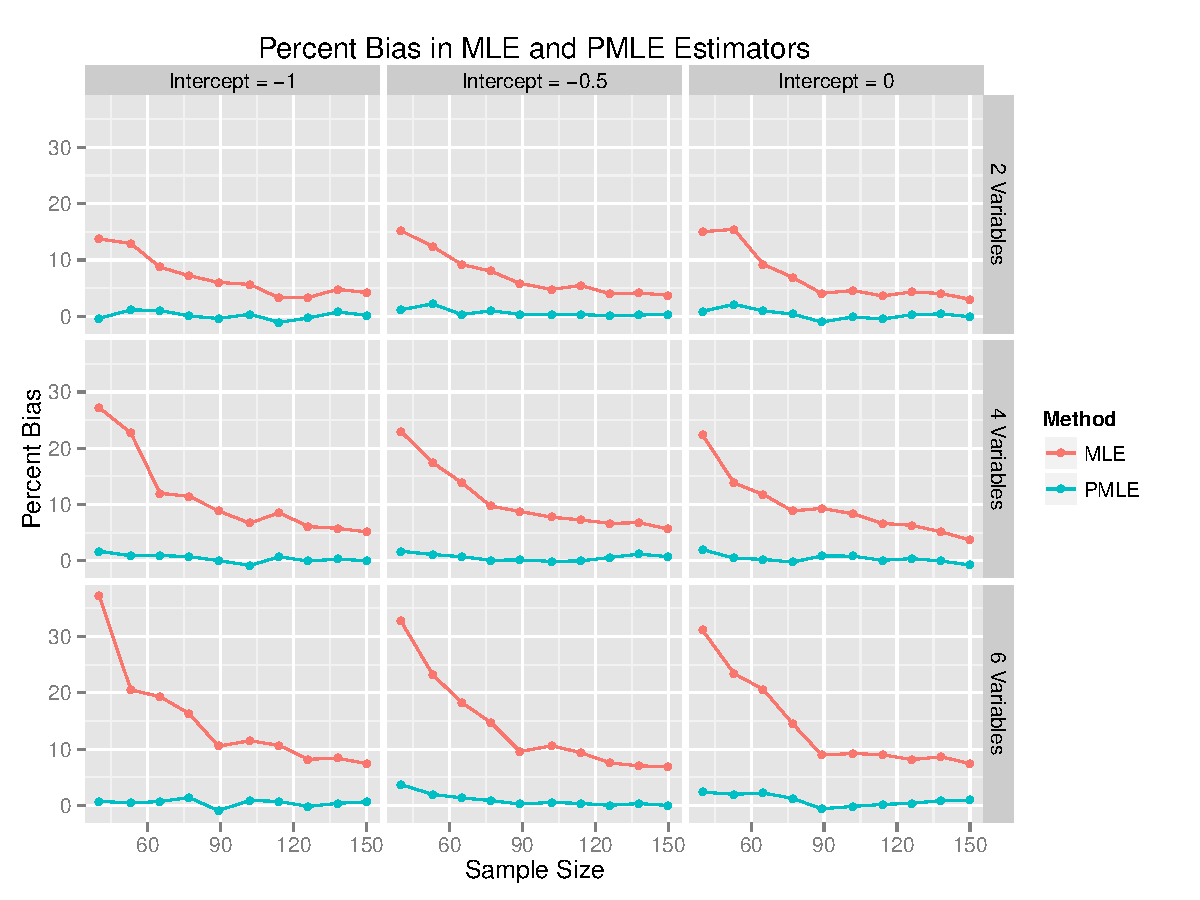
\includegraphics[width = \textwidth]{figs/sims-coef-perc-bias.pdf}
\caption{This figure illustrates the substantial bias of $\hat{\beta}^{mle}$ and the near unbiasedness of $\hat{\beta}^{pmle}$. Notice that when $N = 40$, the bias of $\hat{\beta}^{mle}$ away from zero is about 40\% or more if events are relatively uncommon (e.g., $\beta_0 = -1$, which leads to about 28\% events) or the researcher uses several explanatory variables (e.g., 6 or more). However, notice that $\hat{\beta}^{pmle}$ is essentially unbiased regardless of the sample size, frequency of events, or number of explanatory variables.}\label{fig:sims-coef-perc-bias}
\end{center}
\end{figure}

\subsection*{Variance}

\section*{Replication of Weisiger (2014)}

\citet{Weisiger2014} explains that conquerors in conventional wars cannot expect to win over the defeated population. Additionally, he describes how sometimes violence continues after the official end of the war in the form of guerrilla warfare instead. Weisiger argues that if resistance occurs, it will be where conditions are favorable for insurgency, such as, difficult terrain, the size and concentration of the occupying force, or if there remains a pre-war leader for potential insurgents to rally around. He hypothesizes that there will be a greater chance of resistance when the pre-conflict political leader ``remains at large in the conquered country" (p. 8).

Weisiger's sample consists of 49 observations so the original analysis uses multivariate linear probability regressions to test his hypotheses. He does so in order to avoid problems with separation and biases that may occur with his small sample if he were to use the standard logit or probit analysis. He acknowledges the limitations to using multivariate linear probability regressions in this situation by noting that the method introduces the possibility of estimating non-meaningful predicted probabilities outside the [0, 1] range. We replicate his results and are able to correct the bias of the coefficient estimates using PMLE. Table \ref{tab:coef} shows the coefficient estimates using MLE, PMLE, and the percent change between the two. Notice that MLE substantially over-estimates many of the coefficients 30 percent or more.

\begin{table}
\begin{center}
\caption{MLE and PMLE Comparison}\label{tab:coef}
\begin{tabular}{l c c c}
\hline
               & MLE & PMLE & Percent Change\\
\hline
Constant & $-8.20$ & $-6.54$ & -20 \\
               & $(5.63)$ & $(4.73)$ \\
Conqueror's Polity Score & $-0.10$ & $-0.07$ & -30 \\
               & $(0.10)$ & $(0.09)$ \\
Distance & $1.06$ & $0.80$ &-24 \\
               & $(0.71)$ & $(0.60)$ \\
Terrain & $2.11$ & $1.74$ &-18 \\
               & $(2.49)$ & $(2.23)$ \\
Occupying Army Density & $-0.07$ & $-0.09$ & 31\\
               & $(0.22)$ & $(0.20)$ \\
GDP per capita & $-1.02$ & $-0.58$ & -43 \\
               & $(0.73)$ & $(0.46)$ \\
Coordination & $2.19^{*}$ & $1.72^{*}$ & -21\\
               & $(1.07)$ & $(0.94)$ \\
\hline
%AIC & 49.62 & 50.75 \\
%BIC & 62.87 & 63.99 \\
%Log Likelihood & -17.81 & -18.38 \\
%Deviance & 35.62 & 36.75 \\
%Num. obs. & 49 & 49 \\
\hline
\multicolumn{3}{l}{\scriptsize Notes: {$^*p<0.1$}, standard errors in parentheses.}
\end{tabular}
\end{center}
\end{table}

The use of a logit analysis implies that we are more interested in the functions of the coefficients rather than the coefficients themselves, so we calculated the first differences and the risk ratios for his hypothesis about the presence of the pre-conquest political leader. To do so, we evaluated the difference in the probability of resistance from a situation where there a pre-conquest leader did not remain to a situation where one did remain. We then set the Polity score of the Conqueror to 10, a full democracy, and the rest of the variables at their medians.\footnote{These include: the natural log of the intercapital distance, the type of terrain, the density of the occupying force and the conquered country's per capita GDP.} We did then calculate the first difference and the risk ratio for both the standard MLE and the PMLE.

The values of the quantities of interest of the PMLE decrease in comparison to those of the standard MLE. Using the standard MLE, resistance in a situation where the pre-conquest leader remains is 4.96 times more likely than where the pre-conquest leader does not remain. Using the PMLE, we see the risk ration decrease to 3.25. Similarly, we see the first differences for the same situational change also decrease when using the PMLE instead of the standard MLE. Using the PMLE, the likelihood of resistance in going from a scenario in which the pre-conquest leader remains to one in which none remain decreases by 35 percentage points. With the standard MLE, the likelihood decreases by 40 percentage points. We are then able to calculate our confidence intervals using Clarify or Clarify-like simulations. As with the change in coefficients previously demonstrated in Table \ref{tab:coef}, the changes in the quantities of interest when one uses the PMLE as opposed to the standard MLE, the PMLE corrects for the tendency for coefficients produced by the standard MLE to be biased away from zero.

Because we do not know the true model, we can use out-of-sample predictions as the best way to judge. Table \ref{tab:scores} displays both the Brier and the log scores for the standard MLE and for the PMLE. Both scoring methods indicate that the PMLE is a better predictor than the standard MLE. The Brier score $B$ is calculated as $B = \sum_{i = 1}^n (y_i - p_i)^2$, where $i$ indexes the observations, $y_i \in \{0, 1\}$ represents the actual outcome, and $p_i \in (0, 1)$ represents the estimated probability that $y_i = 1$. The log score is calculated as $\sum_{i = 1}^n log(r_i)$, where $r_i = y_i p_i + (1 - y_i)(1 - p_i)$. 

\singlespace
\begin{table}[H]
\begin{center}
\begin{tabular}{| c | c | c |}
\hline
Estimation Technique & Brier Score & Log Score \\
\hline
MLE & 0.173 & -0.621 \\
PMLE & 0.168 & -0.547 \\
\hline
\end{tabular}\caption{This table compares the Brier and log scores of out-of-sample predictions using MLE and PMLE. Notice that PMLE out-performs MLE according to both measures.}\label{tab:scores}
\end{center}
\end{table}
\doublespace

By replicating \citet{Weisiger2014}, we demonstrate an appropriate way to use logistic regression with small samples. The original study uses multivariate linear probability regressions on a sample of 35 observations to avoid problems with separation and bias. Using a method of penalized maximum likelihood, with the associated risk ratios, first differences, and the Brier and log scores of out-of-sample predictions, we show that the author would be able to make a stronger case for his argument by obtaining more precise estimates by correcting the bias on the coefficients.

\begin{figure}[H]
\begin{center}
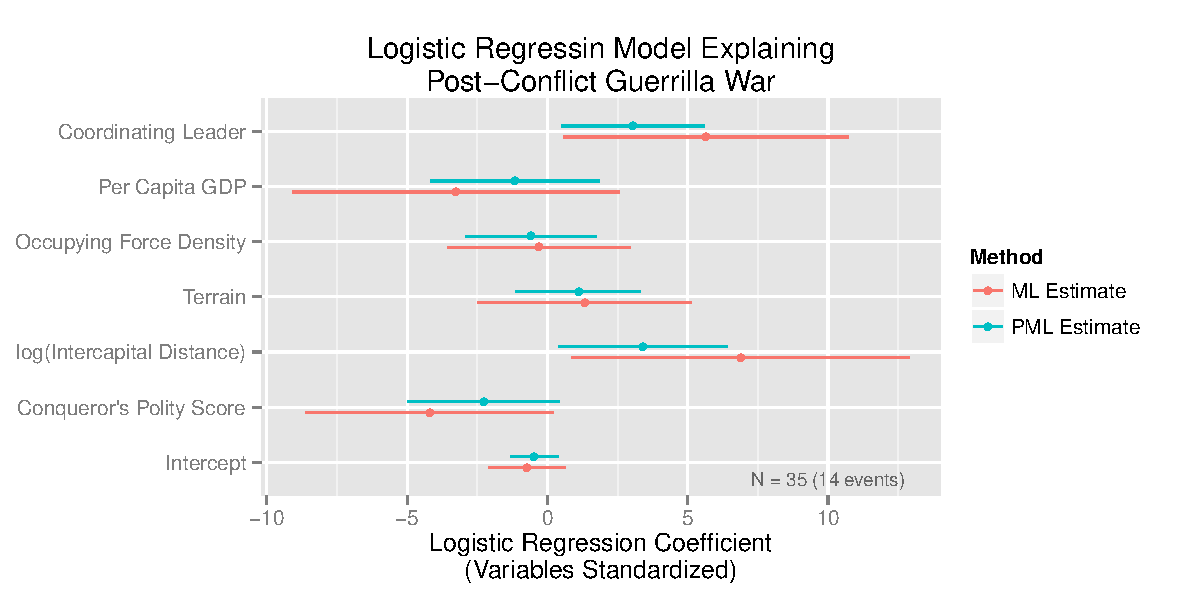
\includegraphics[width = \textwidth]{figs/weisiger-coefs.pdf}
\caption{This figure shows the coefficients for a logistic regression model estimated explaining post-conflict guerrilla war estimated with ML and PML. Notice that the PML estimates tend to be much smaller than the ML estimates.}\label{fig:weisiger-coefs}
\end{center}
\end{figure}

\begin{figure}[H]
\begin{center}
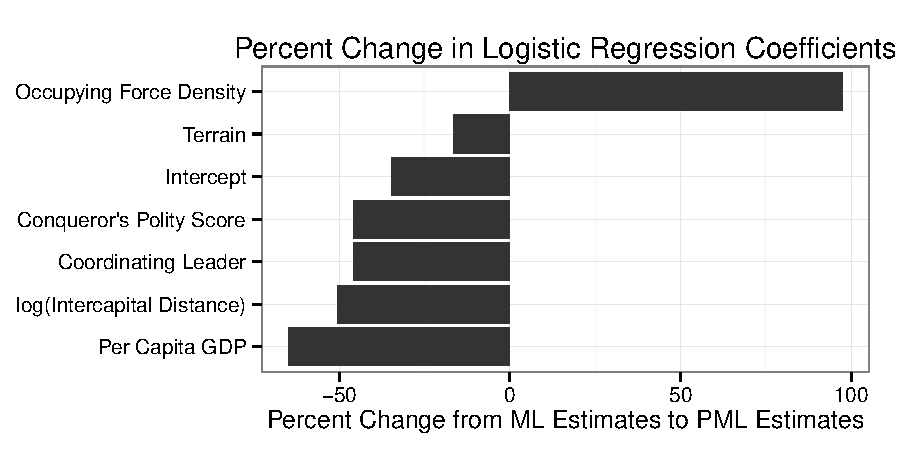
\includegraphics[scale = 1.0]{figs/weisiger-perc-change.pdf}
\caption{This figure shows the percentage change in the logistic regression coefficients in the model of post-conflict guerrilla war from ML to PML. Notice that these changes are substantial--the coefficient for per capita GDP shrinks by over 60\% and the coefficient for occupying force density grows by nearly 100\%. All the coefficients change by more than 45\%, with the exception of terrain, which decreases by 16\%.}\label{fig:weisiger-perc-change}
\end{center}
\end{figure}

\begin{figure}[H]
\begin{center}
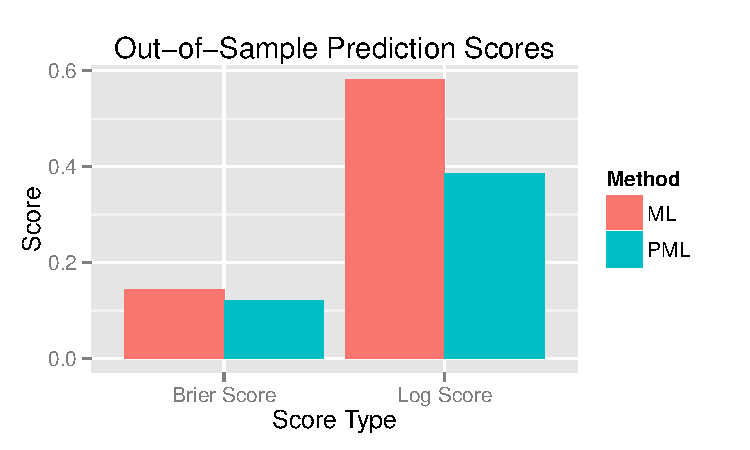
\includegraphics[scale = 1.0]{figs/weisiger-out-sample-fit.pdf}
\caption{This figure shows the out-of-sample predictive ability (leave-on-out cross-validation) of the ML and PML estimators using both Brier and log scores to measure performance. Higher scores indicate better performance. Notice that the PML estimator out-performs the ML estimator according to both scores. This suggests that the ML estimator is overfitting the data.}\label{fig:weisiger-out-sample-fit}
\end{center}
\end{figure}

\begin{figure}[H]
\begin{center}
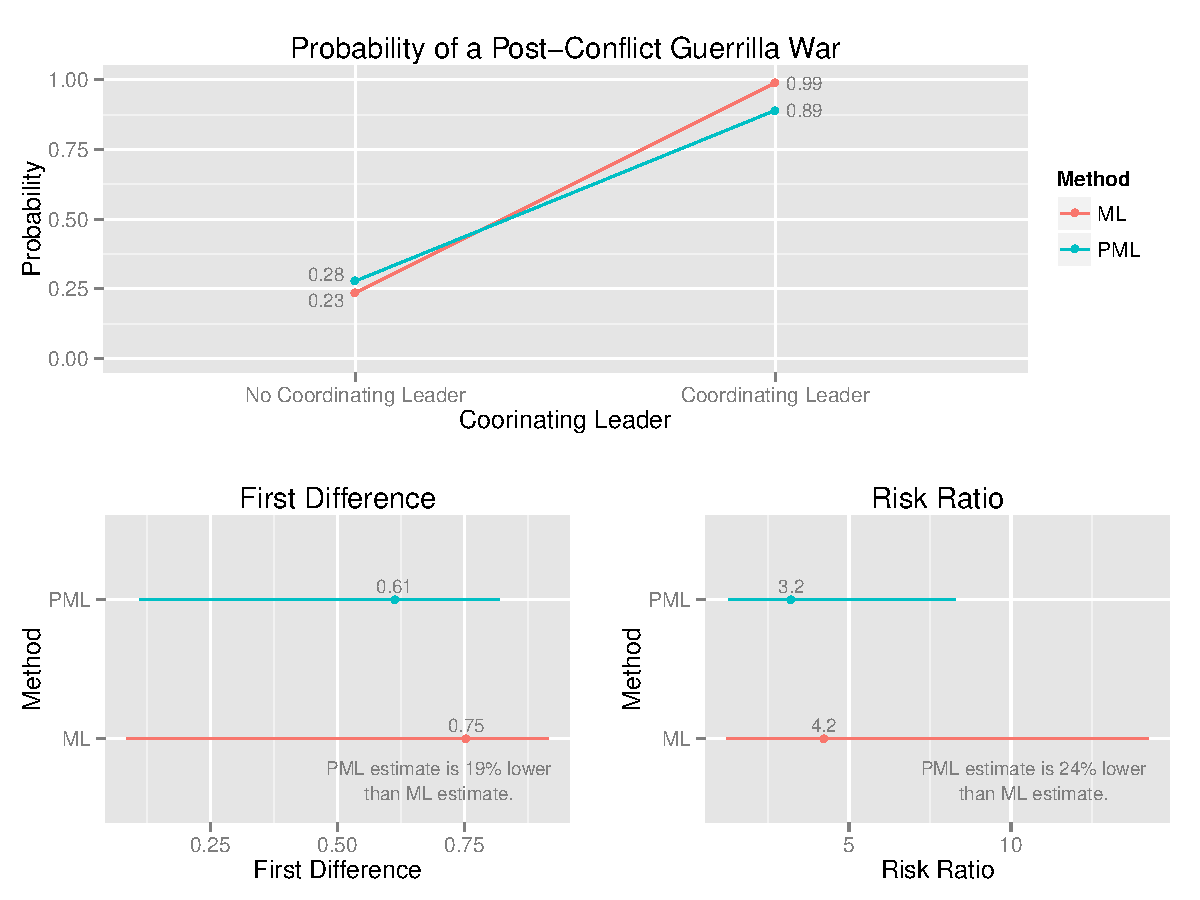
\includegraphics[width = \textwidth]{figs/weisiger-qis.pdf}
\caption{This figure shows the quantities of interest for the effect of a coordinating leader on the probability of a post-conflict guerrilla war. Notice that the PML estimates suggests 19\% smaller first difference and a 24\% smaller risk ratio.}\label{fig:weisiger-qis}
\end{center}
\end{figure}

\singlespace 
\newpage
\normalsize
\bibliographystyle{apsr_fs}
\bibliography{/Users/carlislerainey/Dropbox/papers/bibliography/bibliography.bib}
%\bibliography{/Users/kellymccaskey/Dropbox/Projects/bibliography/bibliography.bib}

\newpage
\begin{appendix}
\begin{center}
{\LARGE Online Appendix}\\
{\large Logistic Regression in Small Samples}\\\vspace{2mm}
\end{center}


\section{Penalized Maximum Likelihood Estimation of Logistic Regression Models in R}\label{sec:pmle-in-R}

\begin{verbatim}

# load data
library(readr)  # for read_csv()
weisiger <- read_csv("weisiger-replication/data/weisiger.csv")

# quick look at data
library(dplyr)  # for glimpse()
glimpse(weisiger)

# model formula
f <- resist ~ polity_conq + lndist + terrain_alt + 
  soldperterr + gdppc2_alt + coord

# ----------------------------- #
# pmle with the logistf package #
# ----------------------------- #

# estimate logistic regression with pmle
library(logistf)  # for logistf()
m1 <- logistf(f, data = weisiger)

# see coefficient estimates, confidence intervals, p-values, etc.
summary(m1)

# logistf does **NOT** work with texreg package
library(texreg)
screenreg(m1)

# see help file for more
help(logistf)

# --------------------------- #
# pmle with the brglm package #
# --------------------------- #

# estimate logistic regression with pmle
library(brglm)  # for brglm()
m2 <- brglm(f, family = binomial, data = weisiger)

# see coefficient estimates, standard errors, p-values, etc.
summary(m2)

# brglm works with texreg package
screenreg(m2)

# see help file for more
help(brglm)
\end{verbatim}



\end{appendix}


\end{document}